\documentclass{standalone}
\usepackage{tikz}
\usetikzlibrary{patterns, positioning}
\usepackage[sfdefault]{ClearSans} %% option 'sfdefault' activates Clear Sans as the default text font
\usepackage[T1]{fontenc}

\begin{document}
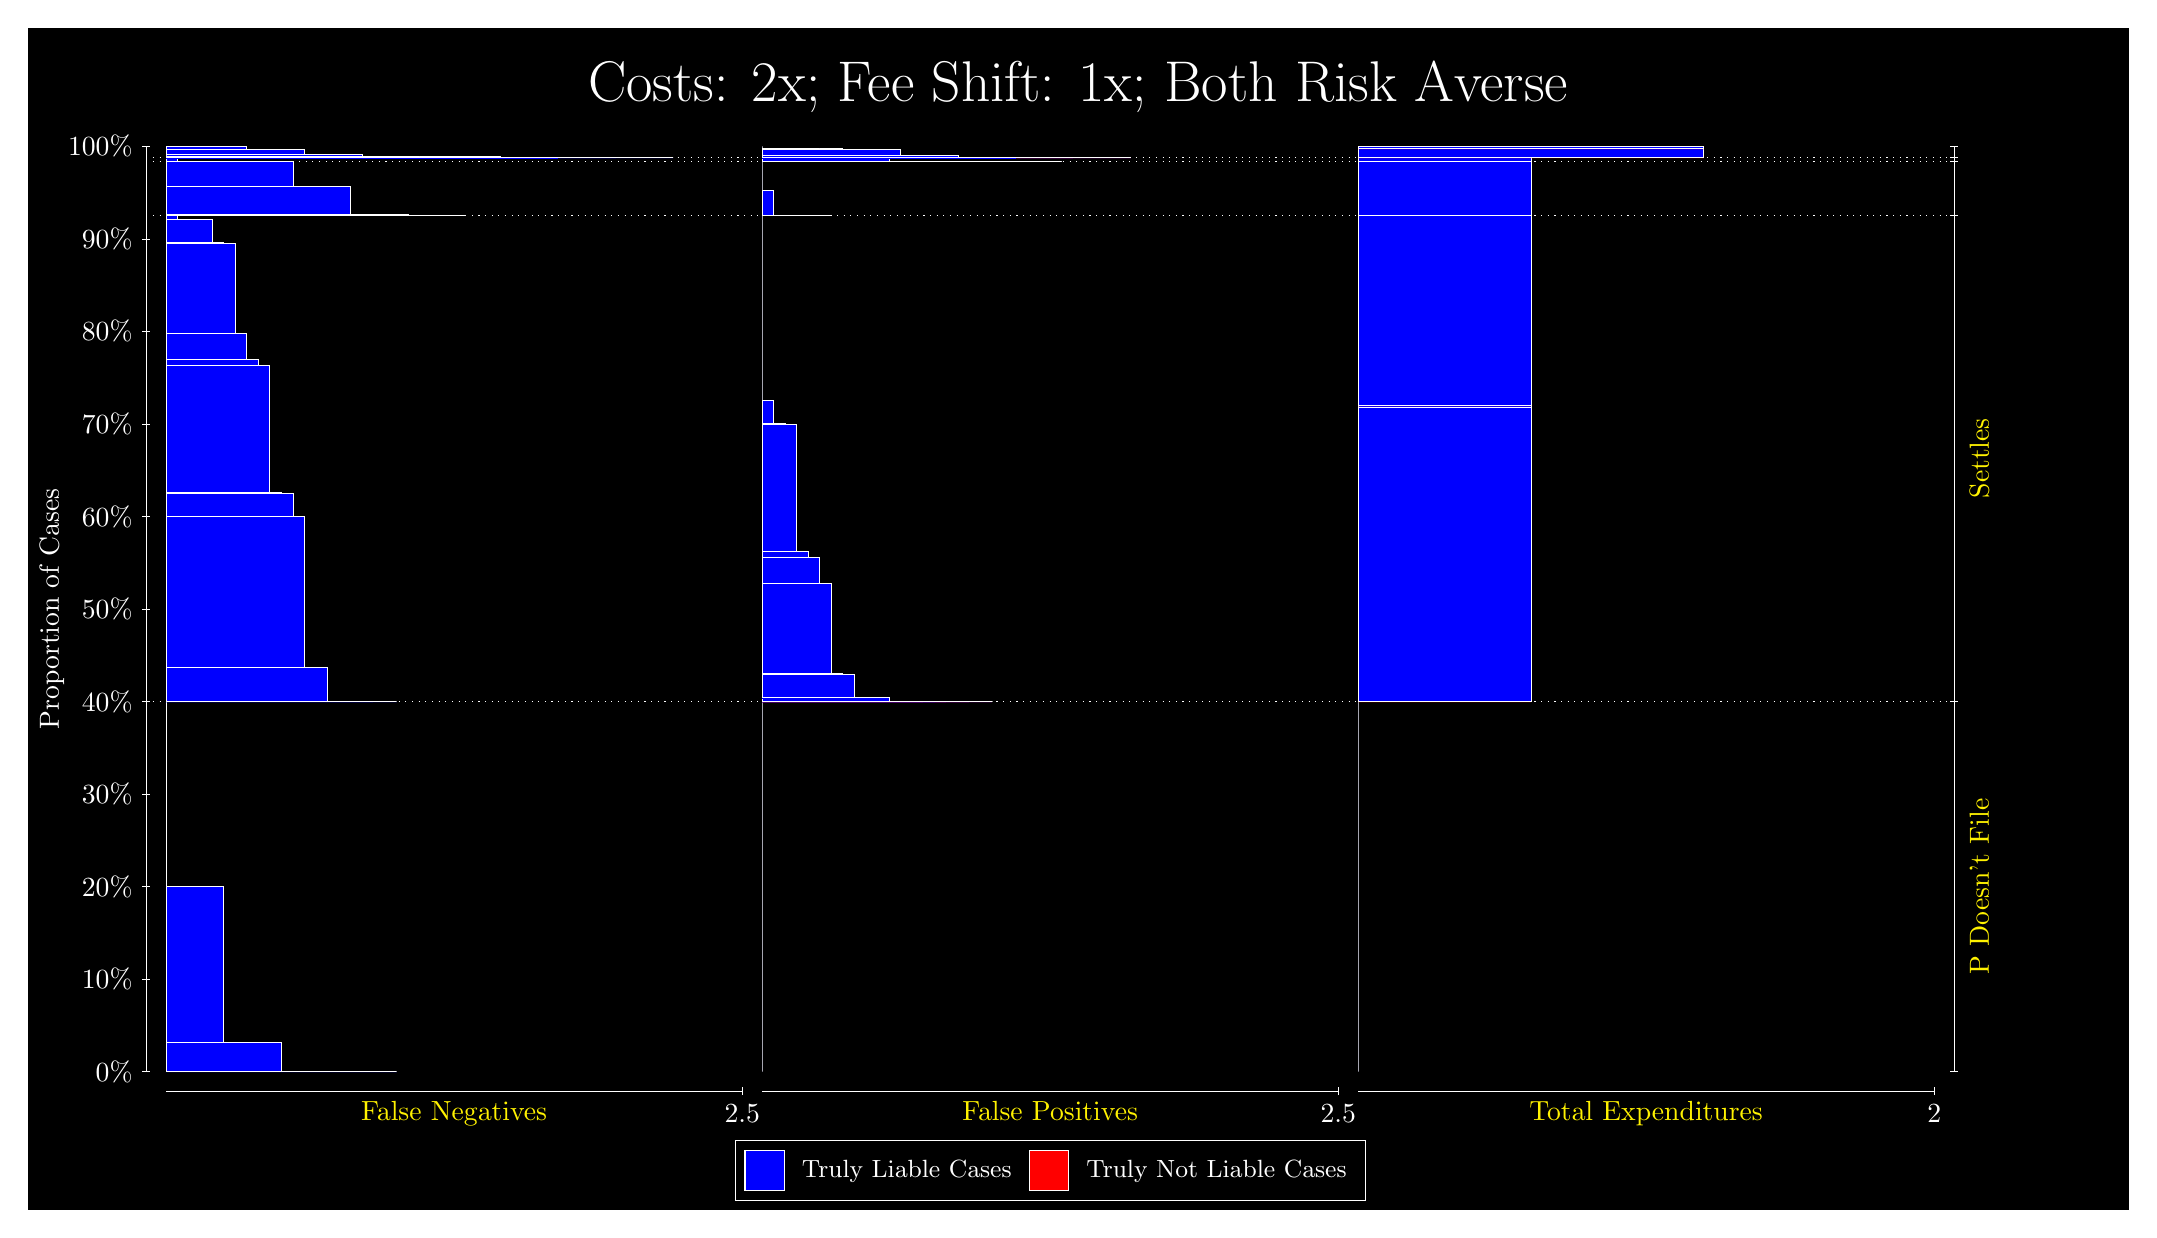
\begin{tikzpicture}
\draw[fill=black] (0,0) rectangle (26.667,15);
\draw[text=white] (0,13.5) rectangle (26.667,15) node[midway] {\huge Costs: 2x; Fee Shift: 1x; Both Risk Averse};
\draw[white, very thin] (1.5,1.75) -- (1.5,13.5);
\node[rotate=90, text=white, anchor=center] at (0.3, 7.625) {Proportion of Cases};
\draw[white, very thin] (1.45,1.75) -- (1.55,1.75);
\node[text=white, anchor=east] at (1.45, 1.75) {0\%};
\draw[white, very thin] (1.45,2.925) -- (1.55,2.925);
\node[text=white, anchor=east] at (1.45, 2.925) {10\%};
\draw[white, very thin] (1.45,4.1) -- (1.55,4.1);
\node[text=white, anchor=east] at (1.45, 4.1) {20\%};
\draw[white, very thin] (1.45,5.275) -- (1.55,5.275);
\node[text=white, anchor=east] at (1.45, 5.275) {30\%};
\draw[white, very thin] (1.45,6.45) -- (1.55,6.45);
\node[text=white, anchor=east] at (1.45, 6.45) {40\%};
\draw[white, very thin] (1.45,7.625) -- (1.55,7.625);
\node[text=white, anchor=east] at (1.45, 7.625) {50\%};
\draw[white, very thin] (1.45,8.8) -- (1.55,8.8);
\node[text=white, anchor=east] at (1.45, 8.8) {60\%};
\draw[white, very thin] (1.45,9.975) -- (1.55,9.975);
\node[text=white, anchor=east] at (1.45, 9.975) {70\%};
\draw[white, very thin] (1.45,11.15) -- (1.55,11.15);
\node[text=white, anchor=east] at (1.45, 11.15) {80\%};
\draw[white, very thin] (1.45,12.325) -- (1.55,12.325);
\node[text=white, anchor=east] at (1.45, 12.325) {90\%};
\draw[white, very thin] (1.45,13.5) -- (1.55,13.5);
\node[text=white, anchor=east] at (1.45, 13.5) {100\%};

\draw[white, very thin] (24.457,1.75) -- (24.457,13.5);
\draw[white, very thin] (24.407,1.75) -- (24.507,1.75);
\node[anchor=west] at (24.407, 1.75) {};
\draw[white, very thin] (24.407,6.4489) -- (24.507,6.4489);
\node[anchor=west] at (24.407, 6.4489) {};
\draw[white, very thin] (24.407,12.627) -- (24.507,12.627);
\node[anchor=west] at (24.407, 12.627) {};
\draw[white, very thin] (24.407,13.311) -- (24.507,13.311);
\node[anchor=west] at (24.407, 13.311) {};
\draw[white, very thin] (24.407,13.355) -- (24.507,13.355);
\node[anchor=west] at (24.407, 13.355) {};
\draw[white, very thin] (24.407,13.5) -- (24.507,13.5);
\node[anchor=west] at (24.407, 13.5) {};

\draw[white, very thin, fill=blue] (1.75,1.75) rectangle (4.6775,1.75);
\draw[white, very thin, fill=blue] (1.75,1.75) rectangle (3.9457,1.7532);
\draw[white, very thin, fill=blue] (1.75,1.7532) rectangle (3.2138,2.126);
\draw[white, very thin, fill=blue] (1.75,2.126) rectangle (2.4819,4.1027);
\draw[white, very thin, fill=red] (1.75,4.1027) rectangle (1.75,4.1027);
\draw[white, very thin, fill=blue] (1.75,4.1027) rectangle (1.75,6.4489);
\draw[white, very thin, fill=blue] (1.75,6.4489) rectangle (4.6775,6.4489);
\draw[white, very thin, fill=blue] (1.75,6.4489) rectangle (4.3848,6.4489);
\draw[white, very thin, fill=blue] (1.75,6.4489) rectangle (4.092,6.4498);
\draw[white, very thin, fill=blue] (1.75,6.4498) rectangle (3.9457,6.4503);
\draw[white, very thin, fill=blue] (1.75,6.4503) rectangle (3.7993,6.8838);
\draw[white, very thin, fill=blue] (1.75,6.8838) rectangle (3.6529,6.8875);
\draw[white, very thin, fill=blue] (1.75,6.8875) rectangle (3.5065,8.7999);
\draw[white, very thin, fill=blue] (1.75,8.7999) rectangle (3.3602,9.0918);
\draw[white, very thin, fill=blue] (1.75,9.0918) rectangle (3.2138,9.1057);
\draw[white, very thin, fill=blue] (1.75,9.1057) rectangle (3.0674,10.719);
\draw[white, very thin, fill=blue] (1.75,10.719) rectangle (2.921,10.79);
\draw[white, very thin, fill=blue] (1.75,10.79) rectangle (2.7746,11.128);
\draw[white, very thin, fill=blue] (1.75,11.128) rectangle (2.6283,12.273);
\draw[white, very thin, fill=blue] (1.75,12.273) rectangle (2.4819,12.278);
\draw[white, very thin, fill=blue] (1.75,12.278) rectangle (2.3355,12.572);
\draw[white, very thin, fill=blue] (1.75,12.572) rectangle (2.1891,12.576);
\draw[white, very thin, fill=blue] (1.75,12.576) rectangle (2.0428,12.577);
\draw[white, very thin, fill=blue] (1.75,12.577) rectangle (1.8964,12.626);
\draw[white, very thin, fill=red] (1.75,12.626) rectangle (1.75,12.626);
\draw[white, very thin, fill=blue] (1.75,12.626) rectangle (1.75,12.627);
\draw[white, very thin, fill=blue] (1.75,12.627) rectangle (5.5558,12.627);
\draw[white, very thin, fill=blue] (1.75,12.627) rectangle (4.8239,12.634);
\draw[white, very thin, fill=blue] (1.75,12.634) rectangle (4.092,12.995);
\draw[white, very thin, fill=blue] (1.75,12.995) rectangle (3.3602,13.307);
\draw[white, very thin, fill=blue] (1.75,13.307) rectangle (2.6283,13.311);
\draw[white, very thin, fill=red] (1.75,13.311) rectangle (1.75,13.311);
\draw[white, very thin, fill=blue] (1.75,13.311) rectangle (2.6283,13.312);
\draw[white, very thin, fill=blue] (1.75,13.312) rectangle (1.8964,13.35);
\draw[white, very thin, fill=red] (1.75,13.35) rectangle (1.75,13.35);
\draw[white, very thin, fill=blue] (1.75,13.35) rectangle (1.75,13.355);
\draw[white, very thin, fill=blue] (1.75,13.355) rectangle (8.1906,13.355);
\draw[white, very thin, fill=blue] (1.75,13.355) rectangle (7.4587,13.355);
\draw[white, very thin, fill=blue] (1.75,13.355) rectangle (6.7268,13.358);
\draw[white, very thin, fill=blue] (1.75,13.358) rectangle (5.9949,13.373);
\draw[white, very thin, fill=blue] (1.75,13.373) rectangle (5.7022,13.373);
\draw[white, very thin, fill=blue] (1.75,13.373) rectangle (5.2631,13.375);
\draw[white, very thin, fill=blue] (1.75,13.375) rectangle (4.9703,13.375);
\draw[white, very thin, fill=blue] (1.75,13.375) rectangle (4.5312,13.375);
\draw[white, very thin, fill=blue] (1.75,13.375) rectangle (4.2384,13.393);
\draw[white, very thin, fill=blue] (1.75,13.393) rectangle (3.7993,13.393);
\draw[white, very thin, fill=blue] (1.75,13.393) rectangle (3.5065,13.465);
\draw[white, very thin, fill=blue] (1.75,13.465) rectangle (2.7746,13.498);
\draw[white, very thin, fill=blue] (1.75,13.498) rectangle (2.0428,13.5);
\draw[white, very thin, fill=red] (1.75,13.5) rectangle (1.75,13.5);
\draw[white, very thin, fill=blue] (1.75,13.5) rectangle (1.75,13.5);
\draw[white, very thin, fill=red] (9.3189,1.75) rectangle (9.3189,1.75);
\draw[white, very thin, fill=blue] (9.3189,1.75) rectangle (9.3189,6.4489);
\draw[white, very thin, fill=red] (9.3189,6.4489) rectangle (12.246,6.4489);
\draw[white, very thin, fill=blue] (9.3189,6.4489) rectangle (12.246,6.4489);
\draw[white, very thin, fill=red] (9.3189,6.4489) rectangle (11.954,6.4489);
\draw[white, very thin, fill=blue] (9.3189,6.4489) rectangle (11.954,6.4489);
\draw[white, very thin, fill=red] (9.3189,6.4489) rectangle (11.661,6.4489);
\draw[white, very thin, fill=blue] (9.3189,6.4489) rectangle (11.661,6.4489);
\draw[white, very thin, fill=blue] (9.3189,6.4489) rectangle (11.515,6.4489);
\draw[white, very thin, fill=red] (9.3189,6.4489) rectangle (11.368,6.4489);
\draw[white, very thin, fill=blue] (9.3189,6.4489) rectangle (11.368,6.4489);
\draw[white, very thin, fill=blue] (9.3189,6.4489) rectangle (11.222,6.4494);
\draw[white, very thin, fill=red] (9.3189,6.4494) rectangle (11.075,6.4494);
\draw[white, very thin, fill=blue] (9.3189,6.4494) rectangle (11.075,6.4494);
\draw[white, very thin, fill=blue] (9.3189,6.4494) rectangle (10.929,6.4981);
\draw[white, very thin, fill=blue] (9.3189,6.4981) rectangle (10.783,6.4998);
\draw[white, very thin, fill=blue] (9.3189,6.4998) rectangle (10.636,6.5036);
\draw[white, very thin, fill=blue] (9.3189,6.5036) rectangle (10.49,6.7972);
\draw[white, very thin, fill=blue] (9.3189,6.7972) rectangle (10.344,6.803);
\draw[white, very thin, fill=blue] (9.3189,6.803) rectangle (10.197,7.9478);
\draw[white, very thin, fill=blue] (9.3189,7.9478) rectangle (10.051,8.2859);
\draw[white, very thin, fill=blue] (9.3189,8.2859) rectangle (9.9044,8.3565);
\draw[white, very thin, fill=blue] (9.3189,8.3565) rectangle (9.758,9.9699);
\draw[white, very thin, fill=blue] (9.3189,9.9699) rectangle (9.6116,9.9838);
\draw[white, very thin, fill=blue] (9.3189,9.9838) rectangle (9.4652,10.276);
\draw[white, very thin, fill=blue] (9.3189,10.276) rectangle (9.3189,12.627);
\draw[white, very thin, fill=red] (9.3189,12.627) rectangle (10.197,12.627);
\draw[white, very thin, fill=blue] (9.3189,12.627) rectangle (10.197,12.63);
\draw[white, very thin, fill=blue] (9.3189,12.63) rectangle (9.4652,12.942);
\draw[white, very thin, fill=blue] (9.3189,12.942) rectangle (9.3189,13.311);
\draw[white, very thin, fill=red] (9.3189,13.311) rectangle (13.125,13.311);
\draw[white, very thin, fill=blue] (9.3189,13.311) rectangle (13.125,13.311);
\draw[white, very thin, fill=blue] (9.3189,13.311) rectangle (12.393,13.311);
\draw[white, very thin, fill=blue] (9.3189,13.311) rectangle (11.661,13.315);
\draw[white, very thin, fill=blue] (9.3189,13.315) rectangle (10.929,13.353);
\draw[white, very thin, fill=blue] (9.3189,13.353) rectangle (10.197,13.355);
\draw[white, very thin, fill=red] (9.3189,13.355) rectangle (14.003,13.355);
\draw[white, very thin, fill=blue] (9.3189,13.355) rectangle (14.003,13.355);
\draw[white, very thin, fill=red] (9.3189,13.355) rectangle (13.271,13.355);
\draw[white, very thin, fill=blue] (9.3189,13.355) rectangle (13.271,13.355);
\draw[white, very thin, fill=red] (9.3189,13.355) rectangle (12.539,13.355);
\draw[white, very thin, fill=blue] (9.3189,13.355) rectangle (12.539,13.357);
\draw[white, very thin, fill=blue] (9.3189,13.357) rectangle (11.807,13.39);
\draw[white, very thin, fill=red] (9.3189,13.39) rectangle (11.807,13.39);
\draw[white, very thin, fill=blue] (9.3189,13.39) rectangle (11.807,13.39);
\draw[white, very thin, fill=blue] (9.3189,13.39) rectangle (11.075,13.461);
\draw[white, very thin, fill=blue] (9.3189,13.461) rectangle (11.075,13.462);
\draw[white, very thin, fill=red] (9.3189,13.462) rectangle (10.783,13.462);
\draw[white, very thin, fill=blue] (9.3189,13.462) rectangle (10.783,13.462);
\draw[white, very thin, fill=blue] (9.3189,13.462) rectangle (10.344,13.47);
\draw[white, very thin, fill=blue] (9.3189,13.47) rectangle (10.344,13.48);
\draw[white, very thin, fill=red] (9.3189,13.48) rectangle (10.051,13.48);
\draw[white, very thin, fill=blue] (9.3189,13.48) rectangle (10.051,13.48);
\draw[white, very thin, fill=blue] (9.3189,13.48) rectangle (9.6116,13.48);
\draw[white, very thin, fill=blue] (9.3189,13.48) rectangle (9.6116,13.48);
\draw[white, very thin, fill=red] (9.3189,13.48) rectangle (9.3189,13.48);
\draw[white, very thin, fill=blue] (9.3189,13.48) rectangle (9.3189,13.5);
\draw[white, very thin, fill=red] (16.888,1.75) rectangle (16.888,1.75);
\draw[white, very thin, fill=blue] (16.888,1.75) rectangle (16.888,6.4489);
\draw[white, very thin, fill=red] (16.888,6.4489) rectangle (19.083,6.4489);
\draw[white, very thin, fill=blue] (16.888,6.4489) rectangle (19.083,10.187);
\draw[white, very thin, fill=red] (16.888,10.187) rectangle (19.083,10.187);
\draw[white, very thin, fill=blue] (16.888,10.187) rectangle (19.083,10.208);
\draw[white, very thin, fill=red] (16.888,10.208) rectangle (19.083,10.208);
\draw[white, very thin, fill=blue] (16.888,10.208) rectangle (19.083,12.627);
\draw[white, very thin, fill=red] (16.888,12.627) rectangle (19.083,12.627);
\draw[white, very thin, fill=blue] (16.888,12.627) rectangle (19.083,13.311);
\draw[white, very thin, fill=red] (16.888,13.311) rectangle (19.083,13.311);
\draw[white, very thin, fill=blue] (16.888,13.311) rectangle (19.083,13.355);
\draw[white, very thin, fill=red] (16.888,13.355) rectangle (21.279,13.355);
\draw[white, very thin, fill=blue] (16.888,13.355) rectangle (21.279,13.469);
\draw[white, very thin, fill=red] (16.888,13.469) rectangle (21.279,13.469);
\draw[white, very thin, fill=blue] (16.888,13.469) rectangle (21.279,13.5);
\draw[white, dotted] (1.5,6.4489) -- (24.457,6.4489);
\draw[white, dotted] (1.5,12.627) -- (24.457,12.627);
\draw[white, dotted] (1.5,13.311) -- (24.457,13.311);
\draw[white, dotted] (1.5,13.355) -- (24.457,13.355);
\draw[white, very thin] (1.75,1.5) -- (9.0689,1.5);
\node[text=yellow, anchor=north] at (5.4094, 1.5) {False Negatives};
\draw[white, very thin] (9.0689,1.45) -- (9.0689,1.55);
\node[text=white, anchor=north] at (9.0689, 1.45) {2.5};

\draw[white, very thin] (9.3189,1.5) -- (16.638,1.5);
\node[text=yellow, anchor=north] at (12.978, 1.5) {False Positives};
\draw[white, very thin] (16.638,1.45) -- (16.638,1.55);
\node[text=white, anchor=north] at (16.638, 1.45) {2.5};

\draw[white, very thin] (16.888,1.5) -- (24.207,1.5);
\node[text=yellow, anchor=north] at (20.547, 1.5) {Total Expenditures};
\draw[white, very thin] (24.207,1.45) -- (24.207,1.55);
\node[text=white, anchor=north] at (24.207, 1.45) {2};

\node[text=yellow, centered, rotate=90] at (24.777, 4.0995) {P Doesn't File};
\node[text=yellow, centered, rotate=90] at (24.777, 9.5378) {Settles};




\draw (12.978300999999998,1.5) node[draw=none] (baseCoordinate) {};
\begin{scope}[align=center]
        \matrix[scale=0.5, draw=white, below=0.5cm of baseCoordinate, nodes={draw}, column sep=0.1cm]{
            \node[rectangle, draw, minimum width=0.5cm, minimum height=0.5cm, fill=blue] {}; &
            \node[draw=none, font=\small, text=white] (B) {Truly Liable Cases}; &
            \node[rectangle, draw, minimum width=0.5cm, minimum height=0.5cm, fill=red] {}; &
            \node[draw=none, font=\small, text=white] (B) {Truly Not Liable Cases}; \\
            };
\end{scope}

\end{tikzpicture}
\end{document}